\part{Seminar 3 - 2-D Exact Analytical Model for Surface Mounted Permanent-Magnet Motors With Semi-Closed Slots}

\makebox[.25\textwidth]{Andries Maxime}\makebox[.25\textwidth]{Dallenogare Antoine}\makebox[.25\textwidth]{Mannella Matthias}\makebox[.25\textwidth]{Paul Arthur}

\section{Introduction}
\textbf{Objective}
\begin{itemize}
    \item Study the influence of the slot-opening on the cogging torque and the motor performances
\end{itemize}   

\textbf{How}
\begin{itemize}
    \item The paper first use an analytic model determined by solving Maxwell's equations (in each subdomains) with interface conditions:
         \begin{enumerate}
             \item less computationally time consuming than numerical ones and can provide closed-form solutions that give physical insight of the machine.
             \item good tools for first evaluation on the motors performances and for design optimisation
         \end{enumerate}
    \item Numerical method are used to validate the analytic ones
\end{itemize}

\textbf{Good to know :} 
\begin{itemize}
\item The analytic development is the first one of this kind for this type of machine (2011)
\item The cogging torque is the torque due to the interaction between the permanent magnets of the rotor and the stator slots of a permanent magnet machine. (Also known as detent or 'no-current' torque)
\end{itemize}


\section{Motor geometry and assumptions}

\subsection{Geometry}
\begin{figure}[H]
    \centering
    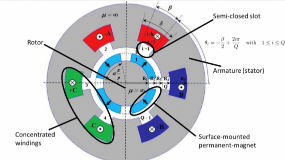
\includegraphics[width = 120mm]{geometry.png}
\end{figure}

\subsection{Hypotheses}
\begin{enumerate}
    \item End effect are neglected
    \item Stator and rotor iron cores are infinitely permeable
    \item The magnets on the rotor are radially magnetised
    \item Relative permeability of the magnets is 1
    \item The stator have radial sides
\end{enumerate}



\section{Mathematical and physical tools}
This section explain the tools needed for the analytic development 
\subsection{Magnetic Vector Potential}
\begin{figure}[H]
    \centering
    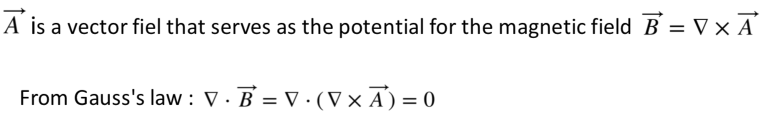
\includegraphics[width = 140mm]{physic/MagVec.png}
\end{figure}

\begin{figure}[H]
    \centering
    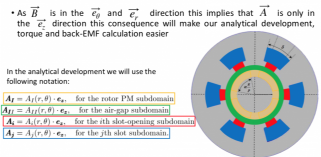
\includegraphics[width = 130mm]{physic/DistribA.png}
\end{figure}

\subsection{Fourier Series expansion}
Just a quick reminder of this tool we use in the analytic development

\begin{figure}[H]
    \centering
    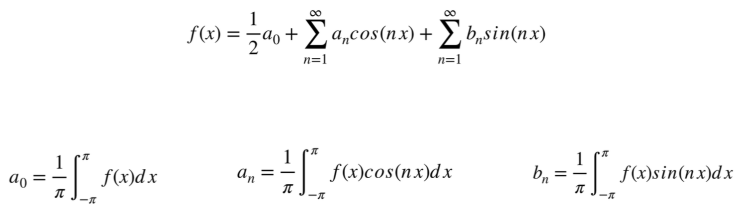
\includegraphics[width = 140mm]{physic/Four.png}
\end{figure}

\subsection{Which equation do we have to solve ?}
We will use the magnetic vector potential because it will simplify the mathematics
\begin{figure}[H]
    \centering
    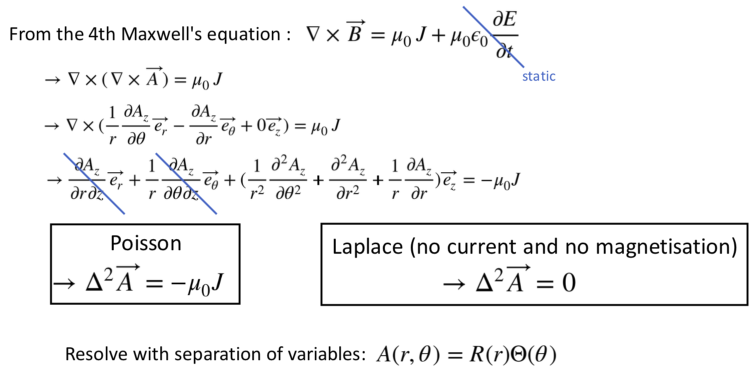
\includegraphics[width = 140mm]{physic/maxeq.png}
\end{figure}

\subsection{In the permanent magnet subdomain}
\begin{figure}[H]
    \centering
    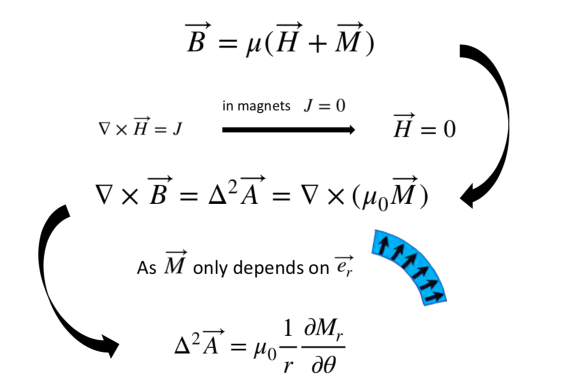
\includegraphics[width = 100mm]{physic/magmax.png}
\end{figure}


\subsection{Interface condition}
\begin{figure}[H]
    \centering
    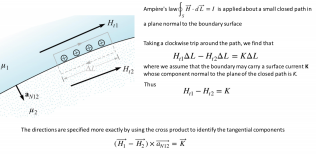
\includegraphics[width = 120mm]{physic/interf.png}
\end{figure}

\subsection{Connecting matrix}
\begin{figure}[H]
    \centering
    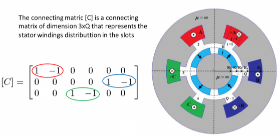
\includegraphics[width = 130mm]{tor/connecting.png}
\end{figure}


\section{Analytical solution of in the different subdomains}

In this section, we will explain how to find the expression of the vector potential A, in the 4 subdomains show below. All this complex calculation will allow us to compute the torque od the machine.

\begin{figure}[H]
    \centering
    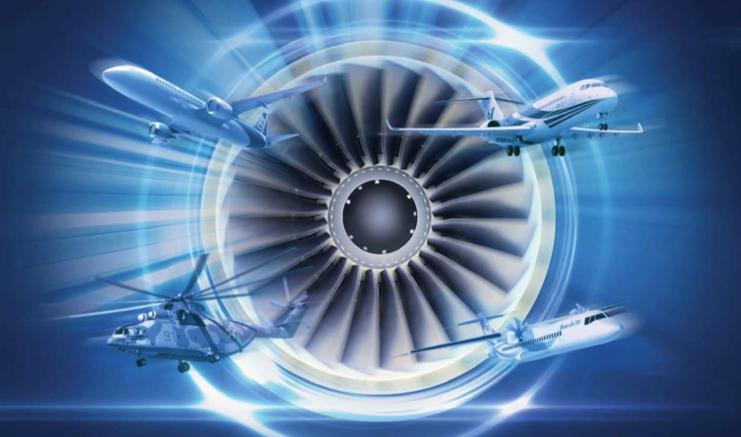
\includegraphics[width = 120mm]{dal/1.png}
\end{figure}

We have 4 domains:
\begin{enumerate}
    \item the $A_i$ subdomains, the slot-opening (air)
    \item the $A_j$ subdomains, the slot with current inside.
    \item the $A_2$ subdomains, the air gap.
    \item the $A_1$ subdomains, the permanent magnet domain (with a magnetisation M)
\end{enumerate}
for each of these domains, we need to find the boundary conditions.

\begin{figure}[H]
    \centering
    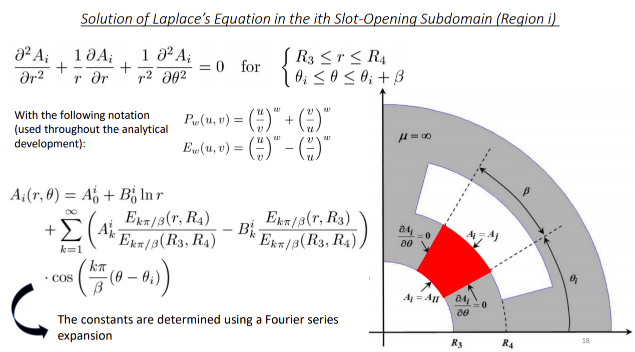
\includegraphics[width = 120mm]{dal/2.png}
\end{figure}
As there is no current trough the surface, the term at left of the equation is null. So we have to slove the laplace equation.
The general solution is given on the slide above. we have 4 constant to find. these will be given on the slide below

\begin{figure}[H]
    \centering
    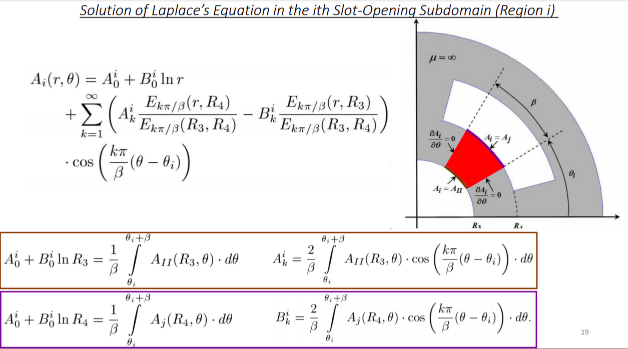
\includegraphics[width = 120mm]{dal/3.png}
\end{figure}
the constant are found with a Fourier series expansion. Let's do the reasoning for the boundary in brown. the mean of our solution should be equal to the mean of the solution found for the air gap. So for a given radius $R_3$, the mean of the solution is $A_0 + B_0\ln{R_3}$ and we can use the integral definition of the mean for the air gap solution. Remember here that we still don't know the air gap solution.
to find the $A_k$ and $B_k$ it's a little bit more complex. So let's do the example for the boundary in brown. When we evaluate the function on $R_3$ only the term $A_k$ is remaining in the big coefficient before the cosine due to the definition of E above. So the remaining equation is an expression of a Fourier series and we can found the Value of $A_k$ at condition to know the value of A on the brown line. So we use the solution of the air gap (that we still don't know) to do this . In fact here, can't solve the system of equations, but we are doing some links between them. It's only when we have done this for the 4 subdomains that we will be able to find all the coefficients. Even in the paper they do not show all the computation, because a computer is needed the find them. We can do the same on $R_4$ and only $B_k$ is remaining in the big coefficient. And here we will use the solution of the domains $A_j$... 

\begin{figure}[H]
    \centering
    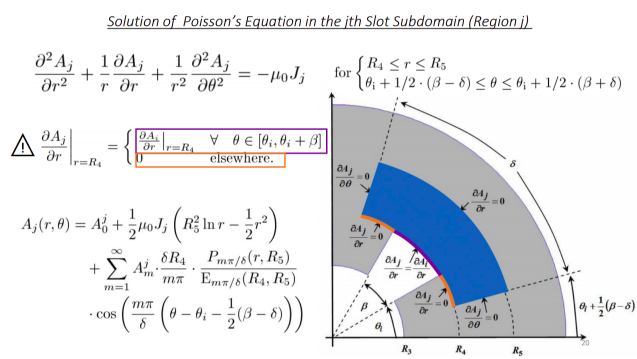
\includegraphics[width = 120mm]{dal/4.png}
\end{figure}

Now we will solve the equation in the subdomain $A_j$. As boundary condition, we ensure that the derivative should be continue between the two subdomain and that next to the iron core, the derivative should be null because of the infinity permeability of the iron core. Here, because of the current density trough the surface, we have a particular solution (the term with the current density J).
\begin{figure}[H]
    \centering
    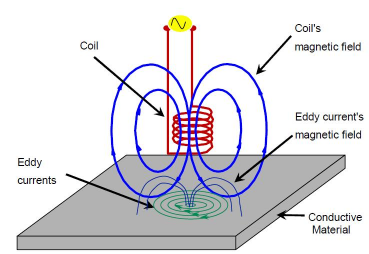
\includegraphics[width = 120mm]{dal/5.png}
\end{figure}
To find the coefficients $A_m$, we can derive the solution and evaluate it on $R_4$. Then, after the computation, only the $A_j$ is remaining before the cosine. So the derivative od the solution have the expression of a Fourier series expansion. So we can compare the solution between the two subdomain like we have done before.

\begin{figure}[H]
    \centering
    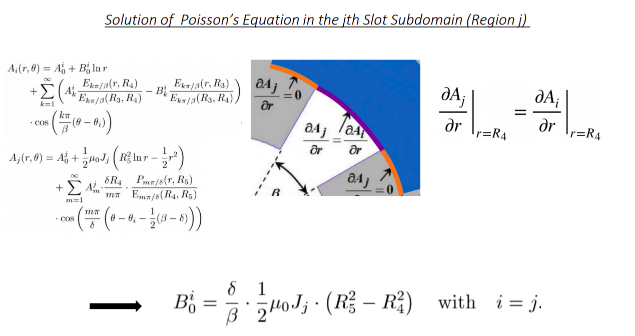
\includegraphics[width = 120mm]{dal/6.png}
\end{figure}

Without using Fourier, and directly the solution, We want to ensure that the mean(on theta) of the two derivatives are the same. (So what's depend on theta is not taken into account -> the infinite summation). So only an equation on $B_0$ is found. $B_0$ is now know. That will be the only coefficient that we can directly know, before solve the entire system. 

\begin{figure}[H]
    \centering
    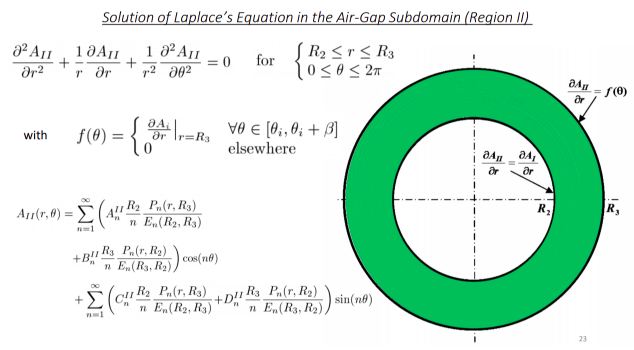
\includegraphics[width = 120mm]{dal/7.png}
\end{figure}
In this domain, there is any boundary in theta. That's why there is any term before the infinite sum. On $R_3$ we have a particular condition that they called f(x). f(x) is introduce because sometime the domain is in contact with the iron core(the derivative is null) or sometime with the slot opening. On $R_2$ the solution should be continue between the two subdomains.    
\begin{figure}[H]
    \centering
    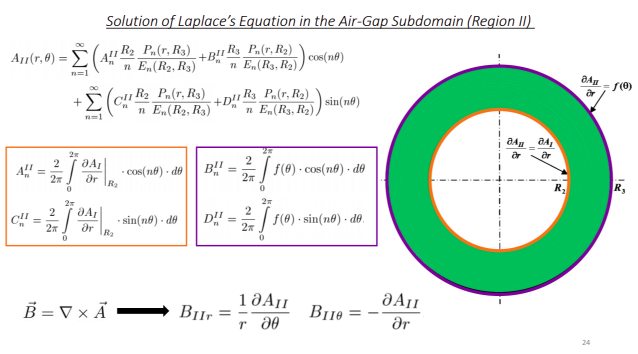
\includegraphics[width = 120mm]{dal/8.png}
\end{figure}
When we evaluate the derivative of the solution on $R_2$, only the coefficients $A_n$ and $C_n$ are remaining before the cosine and before the sinus. We can now use the definition of the Fourier series to make the link between them and the solution in the last subdomain. When we do the same on $R_3$ on can isolate $B_n$ and $D_n$. When A is know is the air gap, we can use it to compute the magnetic field B and then the torque. 
\begin{figure}[H]
    \centering
    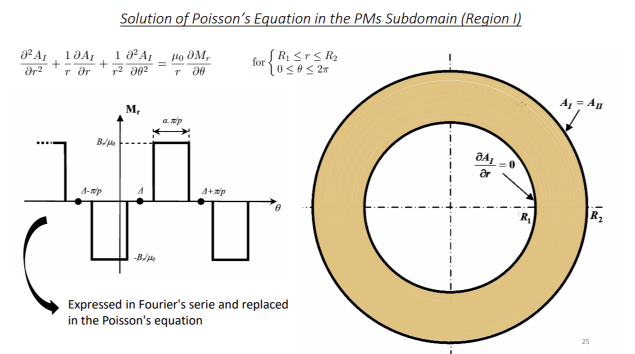
\includegraphics[width = 120mm]{dal/9.png}
\end{figure}
[Remember the slide 13 on the magnetisation]
The magnetisation is shown on the graph. When the signal is positive, we are in a positively magnetised pole and vice versa. We can develop this into Fourier series and replace the result in the equation above. That's how they finf the solution below.

\begin{figure}[H]
    \centering
    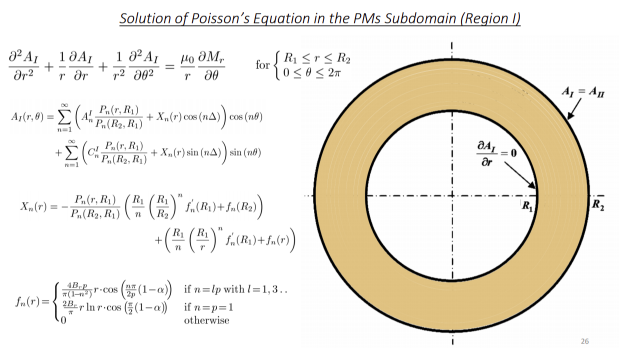
\includegraphics[width = 120mm]{dal/10.png}
\end{figure}
\begin{figure}[H]
    \centering
    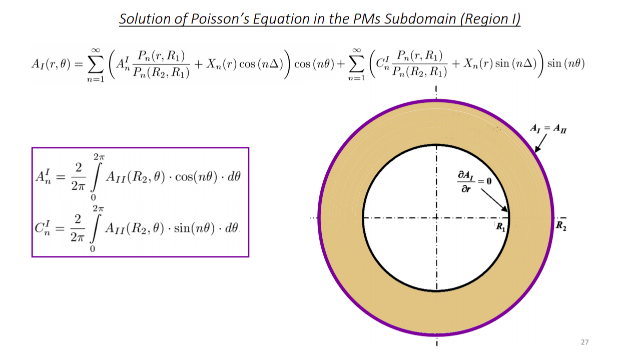
\includegraphics[width = 120mm]{dal/11.png}
\end{figure}
To find the 2 last coefficients, we will use the same technique as before. We evaluate the solution on $R_2$. Then only $A_n$ and $C_n$ will remaining (trust us we have done the development). then we can find the relation between $A_n$ and $C_n$ and the solution of $A_2$

to conclude this part, on have here a really big system of equation that only a computer can solve. Nothing in the paper has been written to explain how do they solve it.

\section{Back EMF and Torque}
\subsection{Electromagnetic torque}
We can use Maxwell equation to rewrite the Lorentz Force that depends on the Maxwell Stress tensor
\begin{figure}[H]
    \centering
    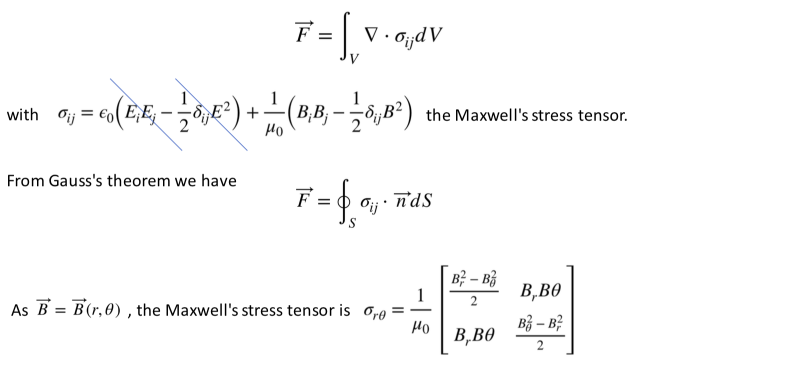
\includegraphics[width = 140mm]{tor/tor1.png}
\end{figure}
\begin{figure}[H]
    \centering
    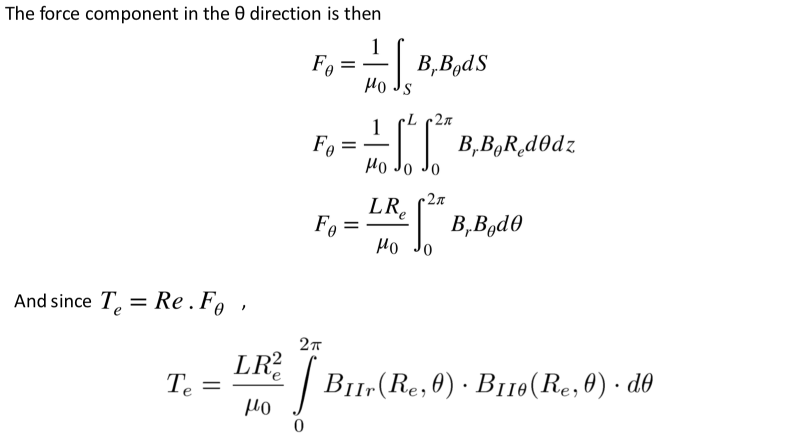
\includegraphics[width = 140mm]{tor/tor2.png}
\end{figure}

There is no interest to develop the last term because it would be too messy and useless. The important think to keep in mind is that the electromagnetic torque depends on the length of the machine, the air gap radius and the magnetic field in this air gap.

\subsection{Back-emf}
\begin{figure}[H]
    \centering
    \includegraphics[width = 150mm]{tor/flux.png}
\end{figure}
We can see that the flux through a surface correspond tho the contour integral on the magnetic vector field potential. 

\begin{minipage}{0.55\linewidth}
We want the flux on just on open-slot so the "contour" to integrate is just the line in blue. If the integral is simply done on the blue line, the expression of the flux is simply: $L \, A_{j}(r, \theta)$
\end{minipage}\hfill
\begin{minipage}{0.4\linewidth}
\begin{figure}[H]
    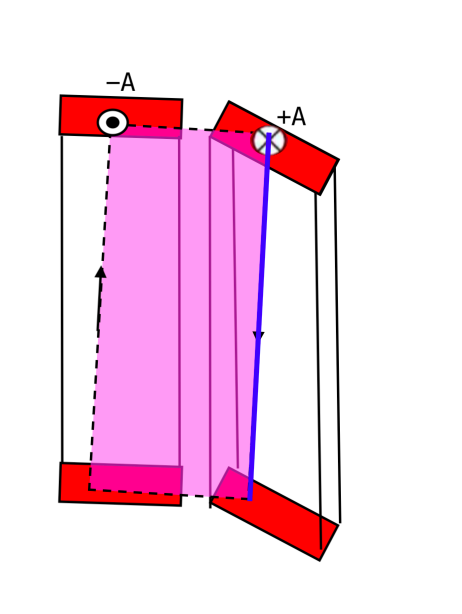
\includegraphics[width = 60mm]{tor/flux2.png}
\end{figure}
\end{minipage}

BUT, as we do not know where the cable is exactly on the slot we use the integral mean theorem  on asurface and then the expression of the flux is 


\begin{minipage}{0.55\linewidth}
\begin{figure}[H]
    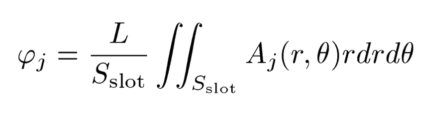
\includegraphics[width = 75mm]{tor/expflux.png}
\end{figure}
\end{minipage}\hfill
\begin{minipage}{0.4\linewidth}
\begin{figure}[H]
    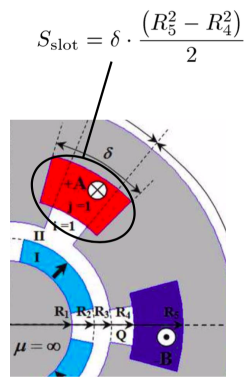
\includegraphics[width = 50mm]{tor/surface.png}
\end{figure}
\end{minipage}

\begin{figure}[H]
    \centering
    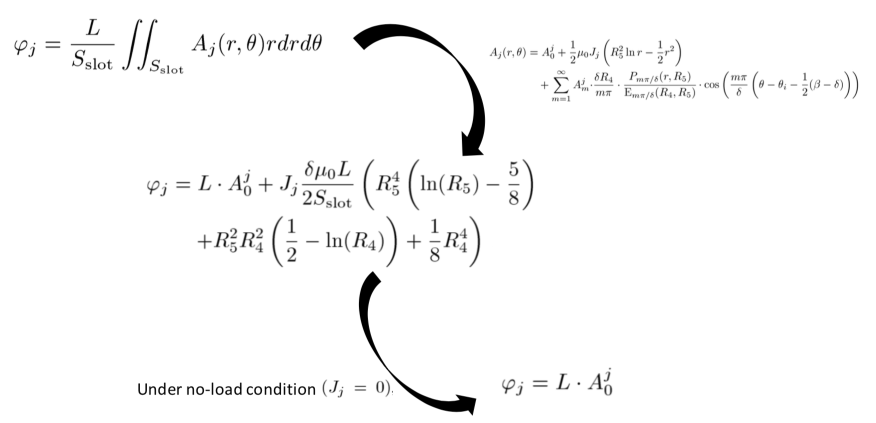
\includegraphics[width = 150mm]{tor/f1.png}
\end{figure}

\begin{figure}[H]
    \centering
    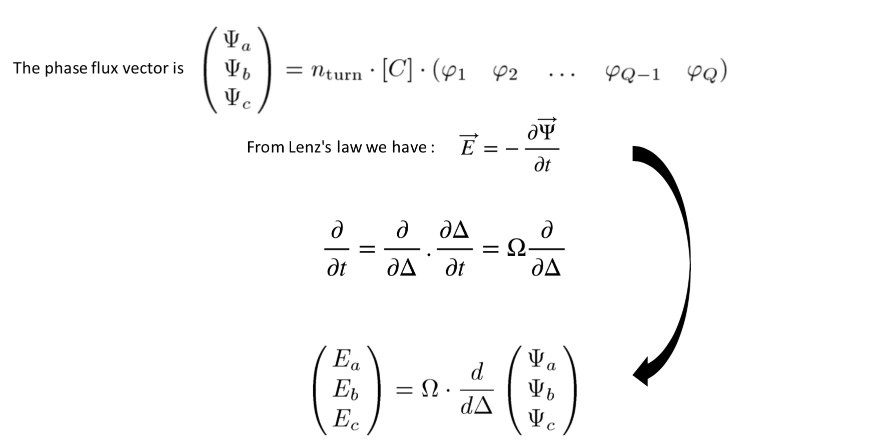
\includegraphics[width = 150mm]{tor/f3.png}
\end{figure}

\section{Analytical results and comparison with FEM (Finite Element Method)}
The analytical results were computed for two differents type of machine:
\begin{itemize}
    \item Fractionnal slots
    \item Integral slots
\end{itemize} 
$$q = \frac{slot}{pole*phase}$$ gives us the type of motor. \\ For both type, the slot opening will introduce high disturbances in the flux at the opening. The results obtained are very similar to the one computed by FEM. We can also see that the cogging torque decreases as the slot opening grows.
\begin{figure}[H]
    \centering
    \includegraphics[width = 150mm]{physic/flux.png}
\end{figure}
\begin{figure}[H]
    \centering
    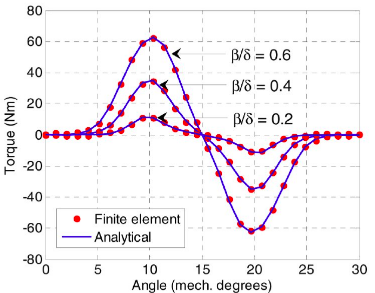
\includegraphics[width = 130mm]{physic/coggingTorque.png}
\end{figure}


\section{Conclusion}
\subsection{Things that we can remember of the paper}
\begin{itemize}
    \item This analytical model is able to predict the electromagnetic torque whatever the value of the slot opening. This result was not possible with the previous models proposed in the litterature
    \item The proposed analytical model is sufficiently general to be used for any pole an slot combinations including fractionnal slot winding machines
    \item Flux density distribution, torque and back-EMF are in close agreement with the finite element computation
    \item The analytical model that was developed can be used to investigate the influence of the design parameters such as slot dimensions, magnet dimensions, slot and pole number combination or windings topologies for the calculation of PM machines performances
\end{itemize}

\subsection{Things we discovered in the paper}
\begin{itemize}
    \item Magnetic vector potential
    \item Fourier's series
    \item Maxwell's stress tensor
    \item Cogging torque
\end{itemize}
